\chapter{FPGA, Microprocesadores Soft-Core y IP-Core}
\section{FPGAs}
	\subsection{Introducción}
	La fabricación de dispositivos semiconductores es un proceso complicado de plazos largos y costosos. Esto lleva a que los diseños destinados para la 
	implementación en chip de silicio tengan poca oportunidad de ser prototipados antes de que comience la producción en grandes volúmenes. Esto supone
	una gran importancia en las fases de prueba y verificación de un diseño antes de ser fabricado.
	
	Basándose en la predicción de la ley de Moore donde expresa que aproximadamente cada dos años se duplica el número de transistores en un circuito
	integrado\cite{Etiqueta02}, Ross Freeman postuló que los transistores serian menos costoso cada año, haciendo asequible la fabricación de chips
	programables personalizables \cite{Etiqueta03}. La compañía Xilinx, ofreció su primer chip en 1984, que contiene arreglo  celdas lógicas (LCAs),
	programables por el usuario en casi cualquier configuración que requieran. Estos se conocen como (\textit{FPGAs}) .
	
	Las \textit{FPGAs} desempeñan un papel dual, uno como objetivo final de ejecución en un diseño y otro papel como prototipo para la implementación
	definitiva de un diseño. Su capacidad de reconfigurar el diseño parcial o totalmente para su actualización o corrección de errores tiene un costo
	relativamente bajo a diferencia del prototipado sobre ASICs. Actualmente las \textit{FPGA} cuentan con una gran cantidad de recursos disponibles
	(Compuertas lógicas , Bloques de RAM) para implementar diseños digitales complejos. Una desventaja de las \textit{FPGA} es debido a la naturaleza
	inherente de su arquitecturas, los diseños implementados en \textit{FPGA}, comparados con los implementados en ASIC, en general tienen mas area,
	menos porformance y consumen mas energía.
	
	A medida que fue pasando el tiempo las FPGAs fueron disminuyendo su costo y mejoraron la eficiencia en el consumo de energía llevándolas a ser
	consideradas como solución a la implementación de ciertas aplicaciones en lugar de un ASIC. Si los criterios tales como el tiempo de
	comercialización y capacidad de actualización son críticos, con el máximo rendimiento y un consumo reducido de energía, una implementación en FPGA
	puede ser adecuada.
	
	Las FPGAs del presente siglo poco tienen que ver con las primeras aparecidas en los 80, y ofrecen densidades de millones de puertas lógicas además
	de microprocesadores empotrados, interfaces de entrada/salida de alta velocidad, bancos de memoria, multiplicadores hardware, DSPs, etc. El
	resultado final es que las FPGAs de hoy en día permiten implementar una gran variedad de sistemas electrónicos: dispositivos de comunicaciones,
	complejos algoritmos de procesamiento de señal, microprocesadores, etc.

	\subsection{Arquitectura}
    Las \textit{FPGAs} son circuitos integrados digitales que contienen bloques de lógica configurable (CLBs) e interconexiones también configurables entre dichos
	bloques, que permiten al desarrollador programarlas para realizar diversas tareas. Xilinx tiene una estructura básica de matriz simétrica (Figura
	~\ref{fig:compfpga}) que ha sido mantenida en sus modernas familias de FPGA, aumentando con cada nueva familia la capacidad de las CLBs e
	interconexiones.
	
	Los componentes de una \textit{FPGA} de Xilinx (Figura ~\ref{fig:compfpga}) son:

	\begin {itemize}
	\item  Bloques lógicos configurables y Lookup Tables.
	\item  Bloques de entrada y salida.
	\item  Bloques multiplicadores.
	\item  Bloques Manejadores de Clock Digitales.
	\end {itemize}

	\begin{figure}[h!]
 	\begin{center}
   	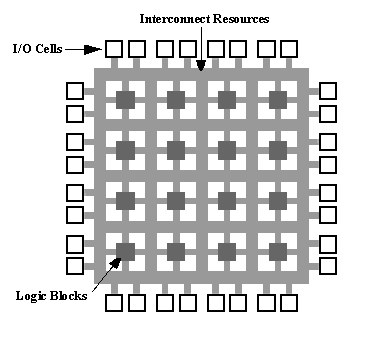
\includegraphics[width=0.5\textwidth,keepaspectratio=true]{./images/fpga1a}
  	\caption{Componentes de una FPGA}
  	\label{fig:compfpga}
 	\end{center}
	\end{figure}

	Otros fabricantes han optado por otro tipo de estructuras internas para sus \textit{FPGAs}, cada una con sus propias ventajas e inconvenientes. No es objeto
	de este trabajo evaluar las estructuras internas de las \textit{FPGAs}.
	
		\subsubsection{Bloques lógicos configurables y lookup tables}
		Todas las\textit{FPGAs} se basan en arrays de pequeños elementos de lógica digital. Los problemas de lógica digital se descomponen en circuitos
		lógicos que puedan ser mapeados a una o más de estas “celdas lógicas” a través de un proceso llamado \textit{“technology mapping"}.
	
		Cada bloque de lógica configurable varía de acuerdo a su fabricante, en el caso de Xilinx tienen el nombre \textit{Logic cell} (LC) (Figura
		~\ref{fig:complc}) contiene una LUT de cuatro entradas, un multiplexor y un registro. Se puede configurar la polaridad del clock, el clock enable y
		la señal de reset.

		\begin{figure}[h!]
		\begin{center}
 		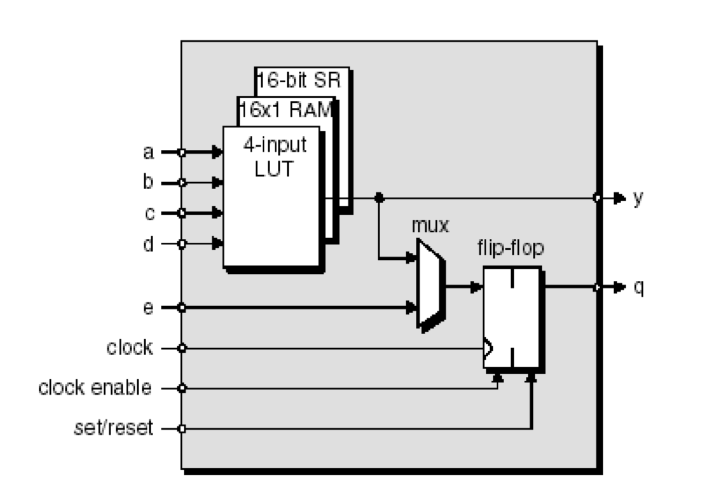
\includegraphics[width=0.5\textwidth,keepaspectratio=true]{./images/celda}
  		\caption{Componentes de una celda lógica}
  		\label{fig:complc}
 		\end{center}
		\end{figure}

		También se encuentran las \textit{Lookup Tables}, que son elementos lógicos que están compuestos de al menos un registro programable (flip\-flop) y
		alguna lógica de entrada, que usualmente está implementada como una \textit{lookup table} de n entradas, donde n es 5 o menos. Estas \textit{LUTs}
		son capaces de implementar cualquier función combinacional de sus entradas.

		\subsubsection{Bloques de entrada y salida de propósito general}
		Las \textit{FPGAs} poseen pines TTL, CMOS, PCI, LVDS y muchos otros que les permiten hacer de interface y convertir tecnologías diferentes.
		Las \textit{FPGAs} tienen bloques de I/O dedicados para clocks y resets globales.
	
		También incluyen PLL y esquemas para el manejo de clocks permitiendo múltiples dominios de los mismos. Las \textit{FPGAs} actuales tienen
		impedancias de I/O configurables, permiten el uso de resistencias internas terminales cuyos valores pueden ser configurados por el usuario.

		\subsubsection{Multiplicadores}
		Algunas funciones como los multiplicadores son muy lentos si se implementan mediante la conexión de un gran numero de bloques lógicos. Por eso
		muchas \textit{FPGAs} incorporan bloques \textit{multiplicadores} hardware (Figura ~\ref{fig:mult}). Estos bloques se encuentran muy cerca de los
		bloques de RAM embebidos.
		
		\begin{figure}[h!]
 		\begin{center}
 		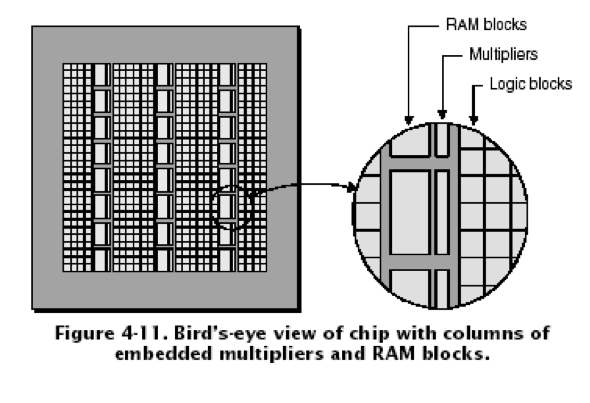
\includegraphics[width=0.5\textwidth,keepaspectratio=true]{./images/multram}
  		\caption{Multiplicadores}
  		\label{fig:mult}
 		\end{center}
		\end{figure}

		\subsubsection{Manejadores de clock digitales}
		El \textit{clock manager} se utiliza para generar un número determinado de “daughter clocks" (Figura ~\ref{fig:dclocks}) . Es utilizado para
		remover el \textit{jitter} como \textit{sintetizador de frecuencia}, donde a partir de una frecuencia de referencia permite obtener un conjunto
		discreto de frecuencias, tratando de mantener en todos los casos las características de estabilidad de la frecuencia de referencia
		\cite{Etiqueta03}, también \textit{phase shifting} algunos diseños requieren clocks que estén corridos en fase unos con respecto a otros.

		\begin{figure}[h!]
 		\begin{center}
 		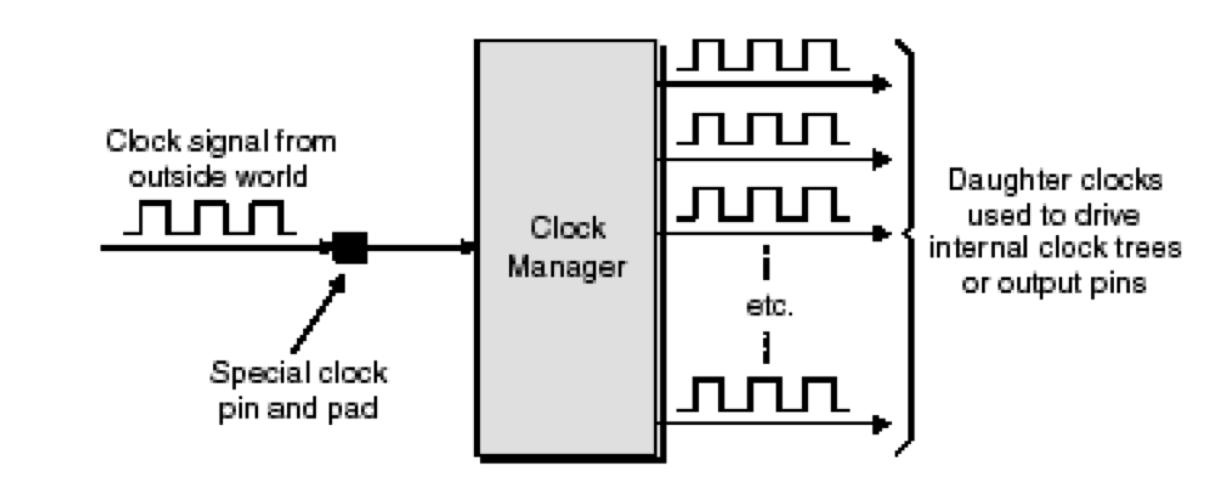
\includegraphics[width=0.5\textwidth,keepaspectratio=true]{./images/dougther}
  		\caption{Clock manager}
  		\label{fig:dclocks}
 		\end{center}
		\end{figure}

		Se tiene  una estructura \textit{clock tree} por la que se distribuye la señal de clock principal, que es ramificada para
		que alcance a todos los flip-flops. Esta estructura es así para asegurar que todos los flip-flop estén lo más cerca posible del clock y evitar el
		problema del \textit{skew}. El \textit{clock tree} es implementado usando canales separados de los de propósito general para interconectar los
		bloques (Figura ~\ref{fig:ctree}).

		\begin{figure}[h!]
 		\begin{center}
 		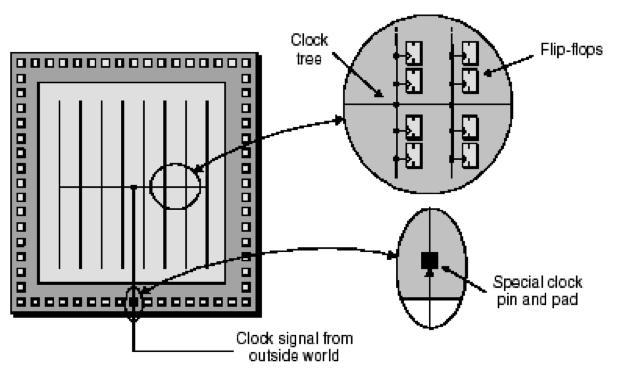
\includegraphics[width=0.5\textwidth,keepaspectratio=true]{./images/clocktree}
  		\caption{Clock tree}
  		\label{fig:ctree}
 		\end{center}
		\end{figure}

	\subsection{Tipo de tecnología} 
	Teniendo en cuenta al tipo de tecnología que utilizan las \textit{FPGAs} para almacenar sus datos de configuración, estas se pueden clasificar en
	tres tipos:

	\begin {itemize}
	\item  
	\textit {Basadas en memoria RAM estática (SRAM)}: Las \textit{FPGAs} guardan su configuración en una memoria interna de tipo SRAM. Cada vez que se
	enciende el sistema es necesario reprogramar la \textit{FPGA} con su configuración, por lo tanto es necesario almacenar esta configuración en un
	dispositivo ROM externo o descargarla desde un PC conectado a la \textit{FPGA}. Este tipo de \textit{FPGA} es la más flexible y permite utilizar
	técnicas de reconfiguración dinámica.
	\item  
	\textit{Basadas en memoria ROM}: Las \textit{FPGAs} almacenan su configuración en una memoria interna de tipo ROM, normalmente FLASH o EEPROM, siendo
	la tecnología FLASH la dominante en estos momentos. La ventaja es que al apagar la \textit{FPGA} la configuración no se pierde, por lo que no son
	necesarios componentes externos para almacenarla. Es menos flexible ya que la configuración es más lenta y no permite utilizar técnicas de
	reconfiguración dinámica.
	\item  
	\textit{Basadas en fusibles}: La configuración se almacena “quemando” fusibles durante el proceso de programación. Actualmente la tecnología más
	utilizada en estas \textit{FPGAs} es la basada en anti-fusibles(anti-fuse). La configuración queda grabada en la \textit{FPGA} de forma que no es
	posible reprogramarla, lo que elimina cualquier tipo de flexibilidad.
 	\end {itemize}

\section{Microprocesadores Softcore Reconfigurables}
	\subsection{Introducción}
	El avance en la tecnología de fabricación de VLSI (Very Large Scale Integration) a medida que se agregaron más y más transistores, y en
	consecuencia más y más funciones fueron integradas en un mismo chip, por lo tanto también las capacidades en FPGAs. Grandes diseños de sistemas
	digitales que fueron sólo para ser implementado como ASICs, luego tuvieron la opción de ser ejecutados en FPGA.
	
	El microprocesador, ya sea como un componente discreto o como parte de otra lógica en el mismo chip, es un buen candidato para ser implementado en
	FPGA. Esto introdujo un mayor potencial para la exploración del espacio de diseño haciendo que la lógica de cómputo específica sea implemetada junto
	con un microprocesador estándar. \cite{Etiqueta05}
	
	Dentro de los microprocesadores \textit{Softcore} se encuentra un grupo que apunta principalmente a la reconfiguración de hardware.
	Tres de los más grandes proveedores de FPGA: Xilinx , Altera y Lattice; ofrecen sus propios núcleos de microprocesadores RISC de 32 bits.
	Existe un grupo de núcleos \textit{Softcore} \textit{Open Source} no limitados por la tecnología. Este grupo es desarrollado por
	lo general por aficionados en comunidades \textit{Open Source}, o en algunos casos, desarrollados por entidades comerciales antes de ser \textit{Open
	Source}.
	
	Para los desarrollos dirigidos a una reconfiguración de hardware la opción de microprocesadores \textit{Softcore} de 32 bits se
 	encuentra entre los que ofrecen los proveedores de FPGA y tambien disponible sin costo dentro de las comunidades \textit{Open Source}. Sin embargo,
 	cuando se trata de ser capaz de desarrollar y vender un producto basado en estos \textit{Cores} \textit{Open Source}, hay consideraciones
 	adicionales sobre la concesión de licencias.
	
	Las verdaderas ventajas de\textit{Softcore Open Source}, tienen que ver con la apertura del diseño, y la ausencia de restricciones sobre lo que se
	puede hacer con el \textit{Core}. Con un diseño de código abierto existe la opción de personalizar la descripción RTL para implementar la
	optimización o la funcionalidad deseada.
	
	La portabilidad y la reutilización del producto final, así como su vigencia por causa del acceso al diseño escrito en lenguaje de descripción de
	hardware también es una de las grandes ventajas de \textit{Softcore Open Source}.

	\subsection{IP-Core}
	El diseño de circuitos digitales se divide normalmente en bloques funcionales, que se refieren como \textit{módulos}, o \textit{cores}. Un
	\textit{core} está formado por sub-bloques que ayudan a poner en práctica su funcionalidad. Los \textit{cores} pueden variar en tamaño hasta el
	tamaño total de un microprocesador. Un \textit{core} puede ocupar una FPGA entera al ser implementado, mientras que sólo se crea una instancia entre
	otros en una FPGA más grande o en un ASIC. Los \textit{núcleos} se describen generalmente utilizando un lenguaje de descripción de hardware (HDL) en
	un nivel de abstracción conocida como Register Transfer Level (RTL).
	
	El proceso de tomar la descripción RTL de un diseño y convertirlo en un lista de primitivas o puertas lógicas y las conexiones entre ellos, dejando
	luego que la  implementación se realice en una tecnología de destino, se conoce como \textit{síntesis}. Análogamente a la compilación de software	que
	se tiene un programa en un lenguaje de alto nivel, como C, y  es convertido a codigo maquina. El resultado de la síntesis, conocida como una
	\textit{netlist}, está en un nivel de abstracción denominado nivel de la puerta.En pocas palabras, es esta lista de conexiones que se utiliza para
	su posterior procesamiento en una configuración para FPGA o en un diseño para ASIC.
	
	Los cores pueden ser diseñados por una persona o entidad, los desarrolladores de \textit{cores} y licenciatarios varían desde particulares
	a empresas. El producto, en este caso se conoce como un \textit{IP core (Intellectual Property Core)} el diseño es la propiedad intelectual de los
	desarrolladores. 
	
		\subsubsection{Tipos de IP-Cores}

		Los \textit{IP cores} se clasifican de acuerdo a su licencia las cuales se presentan a continuación:
		
			\paragraph{Softcores}
			Son los más flexibles y se presentan para \textit{IP} en forma netlist (lista de compuertas e interconexiones) o en forma de sintetizable RTL, lo
			que los hace tecnológicamente independientes.Los \textit{cores} sintetizable se entregan en un lenguaje de descripción de hardware como Verilog o
			VHDL. Óptimos para diferentes aplicaciones, a costas de menor predictibilidad en la implementación y suelen tener un mayor costo y menor desempeño
			de procesamiento.

			\paragraph{Firmcores}
			Los cores firmes están optimizados para ser implementados en una FPGA, arquitectura o dispositivo en particular. Esta optimización puede ser
			realizada por el fabricante o por un tercero. Utilizar este tipo de IP-Cores requiere disponer de cierto nivel de conocimiento de la arquitectura,
			ya que es posible rutear señales físicas y especificar la colocación de los elementos de diseño. Un ejemplo de cores firmes es el procesador
			MicroBlaze de Xilinx.\cite{Etiqueta04}

			\paragraph{Hardcores}
			Están optimizados para una tecnología específica y no pueden ser modificados por el diseñador que los utiliza. Son manifestaciones físicas del
			diseño del core ya que tienen un layout predefinido incluido en la arquitectura. Son los mejores para aplicaciones plug\&play. Si bien son poco
			flexibles, portables y configurables, son muy predictibles (el timing es fijo) y fiables una vez implementados.

		\subsubsection{Clasificación de acuerdo con la integración}
		El aumento de recursos de las FPGAs junto con la amplia disponibilidad de bloques IP ha hecho posible la integración de sistemas completos en la
		propia FPGA y la aparición de una nueva terminología para clasificarlos. Algunos de los términos que se usan para designar este tipo de sistemas
		son:
		\begin {itemize}
		\item 
		\textit{System on Chip (SoC)}:
 		Circuito integrado formado por diversos módulos VLSI con distinta funcionalidad que interconectados entre sí ofrecen una funcionalidad específica
 		para una aplicación.
		\item 
		\textit{System-on-Programable-Chip (SoPC)}: Se aplica este término específicamente cuando el dispositivo utilizado para realizar el SoC es
		reconfigurable.
		\item 
		\textit{Configurable-System-on-Chip (CSoC)}:Mediante este término se definen los sistemas SoC en los que se hace uso de la capacidad de
		reconfiguración de los mismos para aplicaciones de computación reconfigurable. Pueden incluirse bajo la denominación CSoC tanto los sistemas que
		admiten diferentes configuraciones estáticas según ciertos condicionantes, como los que utilizan la reconfiguración parcial dinámica para modificar
		en tiempo de ejecución una sección hardware.
		\item 
		\textit{Multiprocessor-Configurable-System-on-Chip (MCSoC)}: Se aplica esta definición a los sistemas CSoC que incluyen varias unidades procesador
		funcionando de forma simultánea.
 		\end {itemize}

